\documentstyle[11pt,makeidx,times,xspace,example%
              ,epsfig,rotating,texnames,tabularx]{cernman} 
\def\fileversion{v3.07}
\def\filedate{93/07/08} 
\def\docdate {93/07/08}

\newcommand{\Larg}[1]{{\rm\it\mediumseries#1\/}}
\newcommand{\Largb}[1]{\lcb{\rm\it\mediumseries#1\/}\rcb}
\newcommand{\Largs}[1]{\lsb{\rm\it\mediumseries#1\/}\rsb}

\newcommand{\DefC}[1]{\Lcs{#1}}
\newcommand{\DefCm}[2]{\Lcs{#1}\Largb{#2}}
\newcommand{\DefCo}[2]{\Lcs{#1}\Largb{#2}}
\newcommand{\DefCmo}[3]{\Lcs{#1}\Largb{#2}\Largs{#3}}
\newcommand{\DefCom}[3]{\Lcs{#1}\Largs{#2}\Largb{#3}}
\newcommand{\DefCmm}[3]{\Lcs{#1}\Largb{#2}\Largb{#3}}
\newcommand{\DefComm}[4]{\Lcs{#1}\Largs{#2}\Largb{#3}\Largb{#4}}
\newcommand{\DefCmmm}[4]{\Lcs{#1}\Largb{#2}\Largb{#3}\Largb{#4}}
\newcommand{\DefCmmmm}[5]{\Lcs{#1}\Largb{#2}\Largb{#3}\Largb{#4}\Largb{#5}}
\newcommand{\DefCommm}[5]{\Lcs{#1}\Largs{#2}\Largb{#3}\Largb{#4}\Largb{#5}}
\newcommand{\DefCmmmmm}[6]{\Lcs{#1}\Largb{#2}\Largb{#3}\Largb{#4}\Largb{#5}\Largb{#6}}
\newcommand{\DefCommmm}[6]{\Lcs{#1}\Largs{#2}\Largb{#3}\Largb{#4}\Largb{#5}\Largb{#6}}
 
\newenvironment{BCmd}{\flushleft}{\endflushleft}%AS
\newcommand{\BDefC}[1]{\begin{BCmd}\fbox{\DefC{#1}}\end{BCmd}}
\newcommand{\BDefCm}[2]{\begin{BCmd}\fbox{\DefCm{#1}{#2}}\end{BCmd}}
\newcommand{\BDefCo}[2]{\begin{BCmd}\fbox{\DefCo{#1}{#2}}\end{BCmd}}
\newcommand{\BDefCmo}[3]{\begin{BCmd}\fbox{\DefCmo{#1}{#2}{#3}}\end{BCmd}}
\newcommand{\BDefCom}[3]{\begin{BCmd}\fbox{\DefCom{#1}{#2}{#3}}\end{BCmd}}
\newcommand{\BDefCmm}[3]{\begin{BCmd}\fbox{\DefCmm{#1}{#2}{#3}}\end{BCmd}}
\newcommand{\BDefComm}[4]{\begin{BCmd}\fbox{\DefComm{#1}{#2}{#3}{#4}}\end{BCmd}}
\newcommand{\BDefCmmm}[4]{\begin{BCmd}\fbox{\DefCmmm{#1}{#2}{#3}{#4}}\end{BCmd}}
\newcommand{\BDefCmmmm}[5]{\begin{BCmd}\fbox{\DefCmmmm{#1}{#2}{#3}{#4}{#5}}\end{BCmd}}
\newcommand{\BDefCommm}[5]{\begin{BCmd}\fbox{\DefCommm{#1}{#2}{#3}{#4}{#5}}\end{BCmd}}
\newcommand{\BDefCmmmmm}[6]{\begin{BCmd}\fbox{\DefCmmmmm{#1}{#2}{#3}{#4}{#5}{#6}}\end{BCmd}}
\newcommand{\BDefCommmm}[6]{\begin{BCmd}\fbox{\DefCommmm{#1}{#2}{#3}{#4}{#5}{#6}}\end{BCmd}}

\renewcommand{\Lenv}[1]{\mbox{\texttt{#1}}{\index{#1@{\tt#1} environment}}}
\newcommand{\LBEG}[1]{{\rm\tt\bs{}begin\lcb#1\rcb}{\index{#1@{\tt#1} environment}}}
\newcommand{\LEND}[1]{{\rm\tt\bs{}end\lcb#1\rcb}{\index{#1@{\tt#1} environment}}}
\newcommand{\DefE}[1]{\LBEG{#1}}
\newcommand{\DefEm}[2]{\LBEG{#1}\Largb{#2}}
\newcommand{\DefEo}[2]{\LBEG{#1}\Largs{#2}}
\newcommand{\DefEmo}[3]{\LBEG{#1}\Largb{#2}\Largs{#3}}
\newcommand{\DefEom}[3]{\LBEG{#1}\Largs{#2}\Largb{#3}}
\newcommand{\DefEmm}[3]{\LBEG{#1}\Largb{#2}\Largb{#3}}
\newcommand{\DefEmom}[4]{\LBEG{#1}\Largb{#2}\Largs{#3}\Largb{#4}}
\newcommand{\DefEomm}[4]{\LBEG{#1}\Largs{#2}\Largb{#3}\Largb{#4}}
\newcommand{\DefEmoo}[4]{\LBEG{#1}\Largb{#2}\Largs{#3}\Largs{#4}}
\newcommand{\DefEomo}[4]{\LBEG{#1}\Largs{#2}\Largb{#3}\Largs{#4}}
\newcommand{\DefEmmm}[4]{\LBEG{#1}\Largb{#2}\Largb{#3}\Largb{#4}}

%   ......  and their boxed versions
\newcommand{\BDefE}[1]{\begin{BCmd}\fbox{\DefE{#1}}\end{BCmd}}
\newcommand{\BDefEm}[2]{\begin{BCmd}\fbox{\DefEm{#1}{#2}}\end{BCmd}}
\newcommand{\BDefEo}[2]{\begin{BCmd}\fbox{\DefEo{#1}{#2}}\end{BCmd}}
\newcommand{\BDefEmo}[3]{\begin{BCmd}\fbox{\DefEmo{#1}{#2}{#3}}\end{BCmd}}
\newcommand{\BDefEom}[3]{\begin{BCmd}\fbox{\DefEom{#1}{#2}{#3}}\end{BCmd}}
\newcommand{\BDefEmm}[3]{\begin{BCmd}\fbox{\DefEmm{#1}{#2}{#3}}\end{BCmd}}
\newcommand{\BDefEmom}[4]{\begin{BCmd}\fbox{\DefEmom{#1}{#2}{#3}{#4}}\end{BCmd}}
\newcommand{\BDefEomm}[4]{\begin{BCmd}\fbox{\DefEomm{#1}{#2}{#3}{#4}}\end{BCmd}}
\newcommand{\BDefEmoo}[4]{\begin{BCmd}\fbox{\DefEmoo{#1}{#2}{#3}{#4}}\end{BCmd}}
\newcommand{\BDefEomo}[4]{\begin{BCmd}\fbox{\DefEomo{#1}{#2}{#3}{#4}}\end{BCmd}}
\newcommand{\BDefEmmm}[4]{\begin{BCmd}\fbox{\DefEmmm{#1}{#2}{#3}{#4}}\end{BCmd}}

\newcommand{\LMsty}[1]{\texttt{#1}\index{#1@{\texttt{#1} style}}}
\let\Lmsty\LMsty

\newcommand{\eg}{e.g.,\@\xspace} %FMi
\newcommand{\ie}{i.e.,\@\xspace} %FMi
\newcommand{\etc}{etc.\@\xspace} %FMi

\newenvironment{tabledesc}{\begin{quote}\footnotesize}{\end{quote}}

\renewcommand{\DVI}{\texttt{dvi}\index{dvi file}}
\newcommand{\DVIPS}{\texttt{dvips}\index{dvips program}}
\newcommand{\gif}{gif\index{gif}}
\newcommand{\Html}{HTML\index{HTML}}
\renewcommand{\PS}{PostScript\index{PostScript}}
\newcommand{\PTD}{\texttt{ptd}\index{ptd program}}
\newcommand{\SGML}{SGML\index{SGML}}
\newcommand{\URL}{URL\index{URL!Universal Resource Locator}}
\newcommand{\Xmosaic}{Xmosaic\index{Xmosaic!HTML viewer}}

\PScommands% Initialize PS boxes
\makeindex
\hoffset=0mm
\begin{document}
\begin{titlepage}%
\begin{center}
\huge \texttt{cernman}, a CERN style for preparing \\
       computer documentation\footnote{This file
       has version number \fileversion, last
       revised \filedate, documentation dated \docdate.}\\[10mm]
\Large  Michel Goossens\\
        CN Division\\
        CH-1211 Geneva 23 \\
        Switzerland\\
        Email:  \texttt{<goossens@cernvm.cern.ch>}\\[5mm]
\large Printed \today
\end{center}
\vfill
\begin{center}\large\bf Short summary\end{center}

This report describes a \LaTeX{} (major) style file, used at CERN
for writing computer documentation.
It is based on Lamport's\cite{bib-LATEX} ``standard'' \LMsty{report} style.
Some of the basic \LaTeX{} commands and environments are redefined
and several other commands are added.
The New Font Selection Scheme is used throughout, as are several extensions
to \LaTeX{} available on the major archives.
The main emphasis has been put on providing high level commands,
somewhat in the spirit of \SGML, so that typographic and page layout 
conventions can be easily implemented in a coherent and global way.
The quasi-automatic translation from the commands defined in this style
into \SGML{} and \Html{} (\WWW),
and from there into a hierarchical information retrieval 
systems, e.g. hypertext based, is also an important consideration.
The basic idea is to tag all information to a level as detailed as possible
and then to ignore these tags if they are not needed in a given application.
It is important to realize that throwing away non-needed information is
trivial, while looking for needed information, which is absent, is impossible.
\vfill
\end{titlepage}
\pagenumbering{roman}
\setcounter{page}{2}

\tableofcontents

\clearpage
\pagenumbering{arabic}
\setcounter{page}{1}
\chapter{The user commands}

In this first part we describe sectioning and simple
text generating commands, with or without argument, which
you can use with the \LMsty{cernman} style.

For the layout \LMsty{cernman} uses \LaTeX's standard 
\LMsty{report} style.
This has the advantage that the present style file
is more robust with respect to future internal changes to the \LaTeX{} styles.

\section{Sectioning commands}

To provide somewhat more control over the page breaking behaviour at
the boundaries of sections in the text, the higher level sectioning
commands \Lcs{section}, \Lcs{subsection} and \Lcs{subsubsection}
have been given the dual equivalents 
\Lcs{Section}, \Lcs{Subsection} and \Lcs{Subsubsection}.
These latter commands have two mandatory parameters, namely
firstly the space which must still be available on the current page
to contain the title and the beginning of the section and secondly
the title of the section (i.e. the standard parameter
of the original \LaTeX{} commands)

As an example the following command first verifies whether at least 4cm
remain available on the current page. If the answer is positive,
the command acts as a normal \Lcs{section} command, while if the
answer is negative, the current page is ended by issueing a \Lcs{newpage}
command, then on the next page the title is written in the 
conventional way and the section is started.
\begin{verbatim}
\Section{4cm}{Title of the section}
Start of the text of the section...
\end{verbatim}

\section{Array, equations and other goodies}

In order to use the extended functionality of
F. Mittelbach's \Lmsty{array} style, the latter is included by default.

To increase the functionality for handling equations, arrays and figures
various style files are included 
(like \Lmsty{subeqnarray}, \Lmsty{subeqn} and \Lmsty{subfigure};
(see ``\TeX{} at CERN''\cite{bib-TAC} for details).

\LaTeX{} is known for its poor handling of floats. 
All too often you end up with all tables and figures at the
end of your document. 
Sometimes you can can get around the problem by using enough 
\Lcs{clearpage} commands, but a simpler solution is
to take over the placement control of the material and put it
were it should go yourself (of course you must then
be sure that there is enough space available, or else 
you can end with large patches of white space \ldots).
Two enviroments \Lenv{Tabhere} and \Lenv{Fighere} provide the needed
functionality of handling the caption material correctly in the 
case of a table and a figure respectively, in both cases forcing
at the same time the material to be placed {\bf here}, i.e. no
float is generated.

\section{Simple text generating commands}

In order to retain consistency across documents a series
of text generating commands which start a new paragraph 
and may or may not be followed by another start of paragraph
are defined below. 

\BDefC{Action}                    

Typesets the string ``\textbf{Action:}'' to initiate
the description of a routine or command.

\newpage %%%%%%%%%%%%%%%%%%%%%%%%%%%%%%%%%%%%%%%%%%%%%%%%%%%%%%%%%%%

\BDefC{Example}
Typesets the string ``\textbf{Example:}'' to indicate the start of an example.

\BDefC{Examples}
Typesets the string ``\textbf{Examples:}'' to indicate the start of several examples.

\BDefC{Idesc}
Typesets the string ``\textbf{Input parameter description:}''
to indicate the start of the description of input parameters.

\BDefC{Odesc}
Typesets the string ``\textbf{Output parameter description:}''
to indicate the start of the description of output parameters.

\BDefC{Pdesc}
Typesets the string ``\textbf{Parameter description:}''
to indicate the start of the description of routine parameters.

\BDefC{Remark}
Typesets the string ``\textbf{Remark:}'' to indicate the start of an remark.

\BDefC{Remarks}
Typesets the string ``\textbf{Remarks:}'' to indicate the start of several remarks.

\subsection{Text generating commands with arguments}

This section contains a list of simple commands, which allow you 
to ``tag'' text in a document in a generic way, i.e. by specifying what
its function is, rather than its precise formatting.
In some cases the tagged string (or the one specified as an optional
argument) will also be entered in the index.

\BDefCm{Carg}{com-arg} 

Flags the \textbf{use} of the \textbf{command argument} \Larg{com-arg},
\eg \verb!\Carg{MYCARG}! typesets \Carg{MYCARG}.
\index{command!argument!use}\index{argument!command}

\BDefCm{Cargdef}{com-arg}

Flags the \textbf{definition} of the \textbf{command argument} 
\Larg{com-arg},
\eg \verb!\Cargdef{MYCARG}! typesets \Cargdef{MYCARG} and enters \Lit{MYCARG}
also into the index as an argument defining entry. 
There should only be one such defining entry per argument in a document.
\index{command!name!definition}\index{name!command}

\BDefCm{Cdef}{com-name}

Flags the \textbf{definition} of the \textbf{command name} \Larg{com-name},
\eg \verb!\Cdef{MYCOM}! typesets \Cdef{MYCOM} and enters \Lit{MYCOM}
also into the index as a defining entry. There should be only 
one defining entry in a document.
\index{command!name!definition}\index{name!command}

\BDefCom{Cind}{idxname}{com-name}

Flags the \textbf{use} of the \textbf{command name} \Larg{com-name}.
The mandatory argument \Larg{com-name} will by typeset in the text and also in 
the index as a reference to the command name in question. 
If the optional argument \Larg{idxname}
is specified, then the latter will be used as the index entry.
Either of the two strings can be empty, with the expected result.
For instance if you want to flag an entry \textbf{without}
putting it into the index, you can use \verb!\Cind[]{cmdname}!,
while \verb!\Cind[idxname]{}! will enter \Lit{idxname} into the index, but
typeset nothing in the text. 
The latter is useful if you want to flag the use of \eg some routines
or commands in an example, and you do not want to enter
these \LaTeX{} commands inside the text of the example itself.
So you can put a series of the latter commands just following the example,
each instance containing the name of a command or routine used
in the example in question.
Finally, \verb!\Cind{MYCOM}! typesets \Cdef{MYCOM} 
and enters \Lit{MYCOM} also into the index as a reference entry.
\index{command!name!use}\index{name!command}


\BDefCm{Copt}{com-opt} 

Flags the \textbf{use} of the \textbf{command (argument) option} \Larg{com-opt},
\eg \verb!\Copt{MYCOPT}! typesets \Copt{MYCOPT}.
\index{command!option!use}\index{option!command}

\BDefCm{Coptdef}{com-arg}

Flags the \textbf{definition} of the \textbf{command (argument) option} 
\Larg{com-opt},
\eg \verb!\Coptdef{MYCOPT}! typesets \Coptdef{MYCOPT} and enters \Lit{'MYCOPT'}
also into the index as an option defining entry. 
There should only be one such defining entry per option in a document.
\index{command!option!definition}\index{option!command}


\BDefCm{Rarg}{rout-arg} 

Flags the \textbf{use} of the \textbf{routine argument} \Larg{rout-arg},
\eg \verb!\Rarg{MYRARG}! typesets \Rarg{MYRARG}.
Note that the word ``routine'' should be understood
in its widest possible meaning, \ie Fortran as meaning Fortran funtion, routine,
or C, Pascal, \etc, procedure.
\index{routine!argument!use}\index{argument!routine}
\index{Fortran}\index{C}\index{Pascal}\index{procedure}\index{function}

\BDefCm{Rargdef}{rout-arg}

Flags the \textbf{definition} of the \textbf{routine argument} 
\Larg{rout-arg},
\eg \verb!\Rargdef{MYRARG}! typesets \Rargdef{ARG} and enters \Lit{MYRARG}
also into the index as an argument defining entry. 
There should only be one such defining entry per argument in a document.
\index{routine!name!definition}\index{name!routine}

\BDefCm{Rdef}{rout-name}

Flags the \textbf{definition} of the \textbf{routine name} \Larg{rout-name},
\eg \verb!\Rdef{MYROUT}! typesets \Rdef{MYROUT} and enters \Lit{MYROUT}
also into the index as a defining entry. There should be only 
one defining entry in a document.
\index{routine!name!definition}\index{name!routine}

\BDefCom{Rind}{idxname}{rout-name}

Flags the \textbf{use} of the \textbf{routine name} \Larg{rout-name}.
The mandatory argument \Larg{rout-name} will by typeset in the text and also in 
the index as a reference to the routine name in question. 
grep Cind If the optional argument \Larg{idxname}
is specified, then the latter will be used as the index entry.
Either of the two strings can be empty, with the expected result.
For instance, \verb!\Rind{MYROUT}! typesets \Rdef{MYROUT} 
and enters \Lit{MYROUT} also into the index as a reference entry.
\index{routine!name!use}\index{name!routine}


\BDefCm{Ropt}{rout-opt} 

Flags the \textbf{use} of the \textbf{routine (argument) option} \Larg{rout-opt},
\eg \verb!\Ropt{MYROPT}! typesets \Ropt{MYROPT}.
\index{routine!option!use}\index{option!routine}

\BDefCm{Roptdef}{rout-arg}

Flags the \textbf{definition} of the \textbf{routine (argument) option} 
\Larg{rout-opt},
\eg \verb!\Roptdef{MYROPT}! typesets \Roptdef{MYROPT} and enters \Lit{'MYROPT'}
also into the index as an option defining entry. 
There should only be one such defining entry per option in a document.
\index{routine!option!definition}\index{option!routine}

\BDefCm{Ucom}{user-com}

The argument \Larg{user-com} corresponds to a command to be
types by the user and it is typeset in a special way to make
it stand out clearly, eg \verb!\Ucom{ftp asis01}! is typeset
as \Ucom{ftp asis01}.

\chapter{More complex commands}

\section{Commands to highlight calling sequences and commands}

This section describes a series of commands for describing
the structure of Fortran routines or function,
C procedures, KUIP commands, \etc
For most of the commands an optional argument allows you 
to enter information
into the left margin, so that commands can be easily located.
The other parameters specify the name of the label with which 
the entity being defined will be cross-referenced in the index,
the next argument the part of the command or sequence to be
highlighted and finally the parameters themselves.
Apart from the optional (first) parameter between square 
brackets, all other parameters, as described below \textbf{must}
be specified. 
In particular, if there are no parameters, the last
parameter to the command should be empty \Lit{\lcb\rcb}.

The general structure of these commands is:

\BDefCommm{Sxxx}{margintext}{labeltext}{maintext}{parameters}

\begin{DLtt}{1234567890}
\item[\Larg{margintext}] This optional parameter specifies the text
                         should be written into the left margin.
\item[\Larg{labeltext}]  Character string to be used to refer
                         to the entity in the text.
\item[\Larg{maintext}]   Character string corresponding to the name of
                         routine/command being defined. 
                         In some cases this string acts
                         also as \texttt{labeltext}.
\item[\Larg{parameters}] List of the parameters which the routine/command has.
\end{DLtt}

\BDefComm{Shubr}{margintext}{Rname}{arguments}

The first \textbf{obligatory} parameter \Larg{Rname}, which is the
routine's name, acts in this
case also as label to be used in a \Lcs{ref} command.
This means that one can reference the page where the given command
is defined as \verb+\pageref{Rname}+.
The routine will also be entered under that name in the index.
In hypertext application, this commands serves as an anchor defining entry
for the routine \Larg{Rname}, and will be referenced by the anchor
referencing commands \Lcs{Rind}.
An example and its typeset result are:

\begin{verbatim}
\Shubr[HBOOK]{HBNT}{(ID,CHTITL,CHOPT)}
\end{verbatim}

\Shubr[HBOOK]{HBNT}{(ID,CHTITL,CHOPT)}

You can reference this entry by \verb!\Rind{HBNT}! (typeset like \Rind{HBNT})
and start talking about the arguments of the routine as \verb!\Rarg{CHOPT}!
(typeset as \Rarg{CHOPT}) and about the option for this \Rarg{CHOPT} 
parameter as \verb!\Ropt{M}! (\eg, \Ropt{M} for memory resident Ntuple).

%\begin{verbatim}
%\Shubrz[margintext]{Rname}{parameters}
%\end{verbatim}
%%
%\Lcs{Shubrz} describes a Fortran subroutine, which should only
%be shown at that point in the text, but for which no index entry
%or \Lcs{label} definition is required. 
%This is sometimes necessary when one wants to show the definition
%of a command in various places, but of course one sets up
%the main pointing reference only at one point in the text.

\BDefCommmm{Shubrii}{margintext}{Rname1}{parameters1}{Rname2}{parameters2}

\Lcs{Shubrii} describes two similar Fortran subroutines
at the same time, with the word \textbf{and} between the two definitions. 
Of course only one marginal comment can be specified
as an optional parameter \Larg{margintext} if needed.
An example and its typeset result are:

\begin{verbatim}
\Shubrii{HBPROX}{(ID,VMX)}{HBPROY}{(ID,VMX)}
\end{verbatim}

\Shubrii{HBPROX}{(ID,VMX)}{HBPROY}{(ID,VMX)}
 
\BDefComm{Sfunc}{margintext}{Fname}{Value=Fname(parameters)}

\Lcs{Sfunc} describes a Fortran function. 
In this case, as there should always be at least one function
parameter, the last parameter is parsed and the part between
the equal sign and the opening bracket will be highlighted.
As in the case of \Lcs{Shubr} the first obligatory parameter
is used as cross-reference tag and entered into the index. 
An example is given below.

\begin{verbatim}
\Sfunc{HEXIST}{LOGVAR = HEXIST (ID)}
\end{verbatim}

\Sfunc{HEXIST}{LOGVAR = HEXIST (ID)}

\BDefCommmm{Sfuncii}{margintext}{Fnam1}{val1=Fnam1(par1)}{Fnam2}{val2=Fnam2(par2)}

\Lcs{Sfuncii}, as \Lcs{Shubrii}, describes two Fortran functions
which are quite similar and whose description is short enough
to fit on one line.
An example is given below.

\begin{verbatim}
\Sfuncii[Hbook]{HI}{VARIAB = HI (ID,I)}{HIJ}{VARIAB = HIJ (ID,I,J)}
\end{verbatim}

\Sfuncii[Hbook]{HI}{VARIAB = HI (ID,I)}{HIJ}{VARIAB = HIJ (ID,I,J)}

\BDefComm{SCubr}{margintext}{Pname}{parameters}

\Lcs{SCubr} describes a C routine. 
Its calling sequence is completely identical to the one of \Lcs{Shubr}.
The only difference is that the word \texttt{CALL}, characteristic
of a Fortran language's calling sequence is not prepended to the
output string.

\BDefCommmm{SCubrii}{margintext}{Pnam1}{pars1}{Pnam2}{pars2}

\Lcs{SCubrii} describes two similar C routines.
Similar remarks as for \Lcs{Shubrii} and \Lcs{SCubr} apply.

\BDefComm{SKUIP}{short\_name}{Cname}{arguments}

\Lcs{SKUIP} describes a KUIP command.
In this case the optional parameter \Larg{short\_name} is the
short name to be used a cross-reference label. This
is usefull if the command is complex, \eg 

\begin{verbatim}
\SKUIP[ADD]{HISTOGRAM/OPERATIONS/ADD}{id1 id2 id3 [c1 c2]}
\end{verbatim}

\SKUIP[ADD]{HISTOGRAM/OPERATIONS/ADD}{id1 id2 id3 [c1 c2]}

References to this command can be made with the \Lcs{Cind} command. 
Therefore it is perhaps better to chose a somewhat more precise 
\Larg{short\_name}, since there might be other commands
which ``add'' something together.

\section{Extended list environments}

\LaTeX's standard list environments have been augmented
by introducing description (definition) lists where the width
of the term can be specified. 
Lists have also been given a ``dense'' version, 
\ie there is less spacing between the items.
The table below gives an overview of these new list environments.

\begin{tabular}{@{}ll}
\multicolumn{1}{c}{\bf Environment} & \multicolumn{1}{c}{\bf Description} \\
\DefEm{DL}{width}                   & Description list with width of 
                                      largest item                        \\
                                    & Text of term is in bold             \\
\DefEm{DLtt}{width}                 & Description list with width of 
                                      largest item                        \\
                                    & Text of term is in teletype font    \\
\DefEm{DLc}{width}                  & Denser version of \Lenv{DL} list    \\
\DefEm{DLctt}{width}                & Denser version of \Lenv{DLtt} list  \\
\DefE{OL}                           & Numbered (ordered) list             \\
\DefE{OLc}                          & Dense numbered (ordered) list       \\
\DefE{UL}                           & Unnumbered (itemize) list           \\
\DefE{ULc}                          & Dense unnumbered (itemize) list     \\
\end{tabular}

\bigskip
Examples of the use of these lists are

\begin{example}
\begin{DLtt}{12345}
  \item[CHOPT] Option chosen
  \item[ID]    Identifier
  \item[IFLAG] Flag
    \begin{DLtt}{1}
      \item[0] Start
      \item[1] Continue
      \item[2] Stop
    \end{DLtt}
\end{DLtt}
\end{example}

\section{(Almost) verbatim environments}

Often it is desirable to show text (computer programs, listings) 
``literally'', \ie ``as typed'', but at the same time it is still
sometimes necessary to be able to use some \LaTeX{} commands inside such an
environment, \eg to highlight some text inside the example.
Short literal text can be tagged with the
\Lcs{Lit} command, \eg 

\begin{example}
\Lit{Literal \textbf{bold} #$%^&*}
\end{example}

For multiple lines two ``example'' environments have been defined,
namely 

\fbox{\begin{tabular}{@{}l}%
  \DefE{XMP}\\
  \DefEm{XMPt}{Example title}
      \end{tabular}}

\medskip

They are inspired by \LaTeX's standard \Lenv{verbatim} environment.
As with the \Lcs{Lit} command, all characters, but \bs{}, \lcb{} and \rcb{} 
are typeset ``as typed'', \ie without having to take special precautions.
Inside the \Lenv{XMP} environments all blanks and empty lines are output as such.

\begin{example}
\begin{XMP}
\Ucom{ftp asis01}
user: \Ucom{anonymous}
\end{XMP}
\end{example}

\begin{example}
\begin{XMPt}{Typing funny characters}
After the empty line we type #$%^&

Above is an \textem{empty} line.
\end{XMPt}
\end{example}

\chapter{Short references for special characters}

Table~\ref{tab:shortref}
shows which control sequences for special characters
are predefined in the \LMsty{cernamn} style.
They should be used in preference to lower level \LaTeX{}
or \TeX{} control sequences when you want to tag the
special function of such a character.
Table~\ref{tab:cnasdocref} shows control sequences to be
used for tagging CN-AS Group's packages.

\begin{Tabhere}
\def\X#1{#1 &\tt\string#1}
\begin{center}
\begin{tabular}{*{10}{l}}
\X\amp   &\X\apos    &\X\Ast      &\X\atsign &\X\bs     \\
\X\bsol  &\X\Circ    &\X\Colon    &\X\commat &\X\dollar \\
\X\excl  &\X\hyphen  &\X\lab      &\X\lcb    &\X\lcub   \\
\X\lpar  &\X\lsb     &\X\lsqb     &\X\lsquo  &\X\num    \\
\X\period&\X\percent &\X\percnt   &\X\quest  &\X\quot   \\
\X\rab   &\X\rcb     &\X\rcub     &\X\rpar   &\X\rsb    \\
\X\rsqb  &\X\rsquo   &\X\sbl      &\X\semi   &\X\sol    \\
\X\Tilde &\X\us      &\X\verbar  
\end{tabular}
\end{center}
\caption{Command sequences for special characters}\label{tab:shortref}
\begin{center}
\begin{tabular}{*{6}{l}}
\X\CERNLIB&\X\CMZ      &\X\COMIS      \\
\X\CSPACK &\X\FATMEN   &\X\GEANT      \\
\X\GKS    &\X\HBOOK    &\X\HEPDB      \\
\X\HIGZ   &\X\HPLOT    &\X\KUIP       \\
\X\MINUIT &\X\PATCHY   &\X\PAW        \\
\X\ZEBRA   \\
\end{tabular}
\end{center}
\caption{Command sequences to tag CNAS packages}\label{tab:cnasdocref}
\end{Tabhere}

\chapter{Special minor styles}

The \CERNLIB{} and \GEANT{} manuals have a somewhat special layout,
since they contain many (over 200) more or less short descriptions
of independent routines.
Therefore a special macro-command was defined in each case to
format these manual pages, tagging the relevant information
for each routine in an adequate way.
These specific commands are grouped in two minor styles,
\Lmsty{cernlib} and \Lmsty{crngeant}, which are described below.

\section{The \protect\Lmsty{cernlib} style}

The \Lmsty{cernlib} style defines command sequences 
for flagging detailed information about every package.
These commands are described below:

\BDefC{Accuracy}                    

Typesets the string ``\textbf{Accuracy:}'' on a line by itself.

\BDefC{Errorh}                    

Typesets the string ``\textbf{Error handling:}'' on a line by itself.

\BDefC{Longwr}                    

Typesets the string ``\textbf{Long Write-up:}'' on a line by itself.

\BDefC{Method}                    

Typesets the string ``\textbf{Method:}'' on a line by itself.

\BDefC{Notes}                    

Typesets the string ``\textbf{Notes:}'' on a line by itself.

\BDefC{Refer}                    

Typesets the string ``\textbf{References:}'' on a line by itself.

\BDefC{Restrict}                    

Typesets the string ``\textbf{Restrictions:}'' on a line by itself.

\BDefC{Source}                    

Typesets the string ``\textbf{Source:}'' on a line by itself.

\newpage

\BDefC{Structure}                    

Typesets the string ``\textbf{Structure:}'' on a line by itself.

\BDefC{Timing}                    

Typesets the string ``\textbf{Timing:}'' on a line by itself.

\BDefC{Usage}                    

Typesets the string ``\textbf{Usage:}'' on a line by itself.

\BDefCm{Cernhead}{Write-up title}

The \Lcs{Cernhead} command starts the description of a new routine,
resetting the page-counters, enters information into index, and
typesets the title heading for the writeup.
This command uses the information defined by the commands below:

\fbox{\begin{tabular}{@{}l}%
  \DefCm{Author}{Author name}  \\
  \DefCm{Authors}{Author names}
      \end{tabular}}

\medskip

You can specify the author(s) of
the routine with the \Lcs{Author} and \Lcs{Authors} commands, \eg
\verb!\Authors {F.Bruyant, M.Maire}!.

\BDefCm{Keywords}{List of keywords}

The \Lcs{Keywords} command allows you to specify keywords
associated to the routine being described.
The keywords are written to an external file and can be used in online
or hypertext versions of the documentation. \eg

\begin{verbatim}
\Keywords{integration, rational, square root}
\end{verbatim}
 
\BDefCm{Language}{language\_name}

This command specifies in which computer language the package/routine
is written, \eg Fortran, C, Assembler, \etc 

\BDefCm{Library}{library\_name}

This command specifies the name of the computer library 
in which the given package/routine can be found, \eg
\Lit{KERNLIB}, \Lit{MATHLIB}.

\BDefCm{Origin}{Source}

With the \Lcs{Origin} command (\GEANT{} only) you can specify the
source where the routine comes from, \eg \verb!\Origin{GEANT3}!.

\BDefCm{Revised}{revision\_date}

This commands specifies the date of the last revision.

\BDefCm{Routid}{Routine\_identifier}

Identifier for routine (\GEANT{} only), \eg \Lit{BASE020}.

\BDefCm{Submitter}{Name\_of\_submitter(s)}

The \Lcs{Submitter} command allows you to specify the name(s)
of the person(s) who submitted the routine(s).

\BDefCm{Submitted}{submission\_date}

This commands specifies the date when the package was submitted,
\eg \verb!\Submitted{01.10.84}!.

\BDefCm{Version}{package\_code\_name}

The \Lcs{Version} command specifies the name
with with the package is identified in the library (\CERNLIB)
(\eg \verb!\Version{BINOM}!) or the version number for \GEANT{}, 
(\eg \verb!\Version{Geant 3.11}!).

As an example, figure~\vref{fig:cernlibexa} shows 
the input and generated output for \CERNLIB{} routine \Lit{B100}

\begin{figure}[p]
  \begin{sideways}
   \begin{minipage}[b]{\textheight}
    \begin{minipage}[b]{.49\textwidth}
    \scriptsize%
    \begin{verbatim}
\Version{BINOM}                     \Routid{B100}
\Keywords{BINOMIAL COEFFICIENT}
\Author{K.S. K\"olbig}              \Library{MATHLIB}
\Submitter{}                        \Submitted{15.02.1989}
\Language{Fortran}                  \Revised{15.03.1993}
\Cernhead{Binomial Coefficient}
Function subprograms \Rind{BINOM} and \Rind{DBINOM} calculate
the binomial coefficient
\[ x \choose k \ = \ 
  \left\{ \begin{array}{ll}
           x(x-1)\ldots(x-k+1)/k! & (k>0) \\
           1                      & (k=0) \\
           0                      & (k<0) \\
          \end{array}                         \right.  \]
for real $x$ and integer $k$.
Function subprogram {\tt KBINOM} calculates the
binomial coefficient only for integer $x=n$.

On CDC and Cray computers, the double-precision version
\Rind{DBINOM} is not available.
\Structure
{\tt FUNCTION} subprograms \\
User Entry  Names: \Rdef{BINOM}, \Rdef{DBINOM}, \Rdef{KBINOM} \\
Files Referenced: {\tt Unit 6}
\Usage
In any arithmetic expression,
\begin{center}
  \Lit{BINOM(X,K)}, \quad \Lit{DBINOM(X,K)} \quad or \quad
  \Lit{KBINOM(N,K)}
\end{center}
has the value of the binomial coefficient. \Rind{BINOM} is 
of type {\tt REAL}, \Rind{DBINOM} is of type 
{\tt DOUBLE PRECISION} and \Rarg{X} has the
same type as the function name. \Rarg{KBINOM}, \Rarg{N} and 
\Rarg{K} are of type {\tt INTEGER}.
\Restrict
Function subprogram \Rind{KBINOM} can compute only binomial
coefficients which lie in the integer range of the machine.
\Accuracy
Full machine accuracy.
\Errorh
If the result of \Rind{KBINOM} would lie outside the integer 
range ofthe machine, \Rind{KBINOM} is set equal to zero and 
an error message is printed.  \newline
$\bullet$
\end{verbatim}
\end{minipage}
\hfill
\begin{minipage}[b]{.49\textwidth}
\epsfig{bbllx=50pt,bblly=50pt,bburx=550pt,bbury=800pt,clip=,%
        file=b100.eps,width=\textwidth}
\end{minipage}
\caption{Example of using the \protect\Lmsty{cernman} 
         and \protect\Lmsty{cernlib} styles}
\label{fig:cernlibexa}
\end{minipage}
\end{sideways}
\end{figure}

\section{The \protect\Lmsty{crngeant} style}

The \Lmsty{crngeant} minor style includes all the commands
of \LMsty{cernman} and \Lmsty{cernlib}.
As the layout for the description of the individual
routines in the \GEANT{} manual 
is somewhat different from the one of the
\CERNLIB{} short writeups, a different command,
\Lcs{Makehead}  (instead of \Lcs{Cernhead}) should
be used:

\BDefCm{Makehead}{Heading title}

An example of the beginning  of the description
of \GEANT{} routine \Lit{BASE020} is shown below.

\begin{verbatim}
\Authors {F.Bruyant,M.Maire}  \Origin{GEANT3}
\Submitted{01.10.84}          \Revised{23.05.91}
\Version{Geant 3.11}          \Routid{BASE020}
\Makehead{The Data Structures and their Relationship}
\begin{figure}[hbt]
....
\end{verbatim}

In order to ease the introduction of certain physical quantities,
the following definitions, which can be used in text
and math mode, are also provided:

\begin{center}
\makeatletter\input crngeant.sty\makeatother
\def\X#1{#1 &\tt\string#1}
\begin{tabular}{*{8}{l}}
\X\UkeV   & \X\UMeV   & \X\UGeV   & \X\UTeV \\
\X\Pe     & \X\Pme    & \X\Pem    & \X\Pep  \\
\end{tabular}
\end{center} 

\chapter{Making online versions -- \protect\WWW}

The major style \Lmsty{cernman} has been
originally optimized to generate the \PS{} version of
the manuals and writeups describing the software
of CN/AS Group.
Therefore, in order to use the same input \LaTeX{} files
in an (almost) unaugmented way also for producing an online
terminal browsable version or a text version with \SGML{}/\Html{}
tags for viewing with an hypertext system,
many of the \LaTeX{} commands and font definitions 
have to be redefined.
This transformation is performed by overloading the  
\Lmsty{cernman} major style (and possibly the \Lmsty{cernlib}
and \Lmsty{crngeant} minor styles) with the minor styles
\Lmsty{cerndoc} and \Lmsty{cernhtml}.
The latter style also introduces the necessary \Html{} tags
and hypertext links into the document.

Instead of transforming the \DVI-file
into \PS{} with the \DVIPS{} program, in the
latter case the program \PTD{} (Post \TeX{} Doc),
is used to generate an ASCII version of the \DVI-file,
which can be viewed or handled by a post-processor to
generate the necessary files and resolve the necessary links 
for the hypertext (\eg \WWW) systems.

\Lmsty{cernhtml} and \Lmsty{cerndoc}
redefine most  commands set up in the \LMsty{cernman} and
its associated styles \Lmsty{crngeant} and \Lmsty{cernlib}
into a form that can be used for an ASCII text or for 
an \Html{} tagged version.

Figure~\vref{fig:cernmanscheme} gives a complete overview of the various files
and programs involved in producing the various forms
of the CN/AS documentation.
At the left you have the various documents, marked up in \LaTeX,
and containing generic tags for flagging document elements. 
These files are run through \LaTeX{} and depending on the
package or output destination, various style files are loaded
together with the generic style file \Lmsty{cernman}.
The bibliography database \Lit{cnasbibl.bib} can be read
by \BibTeX{} and the index generated with \MakeIndex.
In the next step the \DVI-file is translated into \PS{}
with \DVIPS{} or in a text file with \PTD{} for further 
treatment with an awk script for generating the 
\Html{} files or the terminal readable text files.

\section{The \protect\Html{} interface}

The only \Html{} specific addition, which was introduced into
the \LaTeX{} sources of the documents was a command \Lcs{Filename},
which indicates the filename to be given to the part of the text
starting at that point.
In principle the introduction of this information is not needed per se,
but it helps to manage the many hundreds of files generated for \WWW{} 
related to the CN/AS manuals.
The filename information is used by \LaTeX{} (in the \Lmsty{cernhtml}
style) to build the definition part of the hypertext links (anchors).
This information is later extracted in the post-processing stage 
of the ASCII form of the document in question to resolve,
using a shell script \Lit{makewww.sh},\index{makewww.sh@\texttt{makewww.sh}}
the hypertext cross-references.
During this latter stage possible unresolved references generate a
warning message on the user's screen.

If, in certain points of your document, you want to include 
\Html{} specific information (I think you should not, but, for instance,
on the title page you might have to), you can use the
command 

\BDefCm{HTML}{HTML specific text and commands}

The text specified as argument will only be treated when
you specify the \Lmsty{cernhtml} style option.
This command is ignored by the other styles.

If you want to treat some fo your \LaTeX{} source lines only 
when \textem{not} using \Html, the you can use:

\BDefCm{notHTML}{non-HTML text and commands}

\begin{figure}[p]
\begin{sideways}
\begin{minipage}[b]{\textheight}
\begin{center}
  \fbox{\epsfig{figure=cernmanscheme.eps,width=.85\textwidth}}
\end{center}
\caption{Producing CN/AS documentation}
\label{fig:cernmanscheme}
\end{minipage}
\end{sideways}
\end{figure}

\clearpage

\section{A short overview of \protect\Html}

This section presents a short overview of \Html{}, \WWW's 
text processing language. 
\Html{}, the HyperText Markup Language,
 is defined in terms of the ISO Standard Generalized 
Markup Language (SGML). 
The latest version of the \Html{} language specification
can always be found in \WWW{}, by choosing the ``\WWW{} project''
e.g. on the CERN Welcome page, from there go to 
``Technical aspects of \WWW'' and ``Hypertext Markup Language''.

\subsection{A \protect\Html{} document instance}

\begin{XMPt}{Example of a simple \Html{} document}
<HTML>
<TITLE>This is a simple HTML document</TITLE>
<H1>An Example of a level one heading</H1>
This is the first paragraph of level one.
<H2>An example of a second level heading</H2>
This is the first paragraph of level two.
<P>Another paragraph of level two with a list.
<UL>
<LI>This item contains an <A 
    NAME="#my-anchor">anchor definition</A>.
<LI>This item the second item in the list.
</UL>
And here follows an ordered list.
<OL>
<LI>This item references the <A
    HREF="#my-anchor">previous anchor</A>.
<LI>Another item in the list.
</OL>
<P>Let me show you a definition list:
<DL>
<DT>Term 1<DD>Text of description 1.
<DT>Term 2<DD>Text of description 2.
</DL>
</HTML>
\end{XMPt}

The output corresponding to this document will depend on the
viewing program used.
Below you will find the result of viewing this document with two 
\Html{} viewing programs, namely
the terminal oriented program \Lit{www} (Fig.~\ref{fig:htmlexaoutwww}
and the NCSA X-windows \Html-browser \Xmosaic{} (Fig.~\ref{fig:htmlexaoutxmosaic}

\begin{figure}[p]
  \begin{sideways}
    \begin{minipage}[b]{0.999\textheight}%
\begin{minipage}[b]{.39\textwidth}
\begin{XMP}
\small               This is a simple HTML document

           AN EXAMPLE OF A LEVEL ONE HEADING

   This is the first paragraph of level one.

An example of a second level heading

   This is the first paragraph of level two.
   Another paragraph of level two with a list.

      This item contains an anchor definition.
      This item the second item in the list.

   And here follows an ordered list.
      This item references the previous anchor[1].
      Another item in the list.

   Let me show you a definition list:

  Term 1                 Description 1.
  Term 2                 Description 2.

     [End]
1, Quit, or Help:
\end{XMP}
\caption{The output of the example \protect\Html{} source 
         shown by the \protect\Lit{www} program}
\label{fig:htmlexaoutwww}
\end{minipage}\hfill
\begin{minipage}[b]{.59\textwidth}
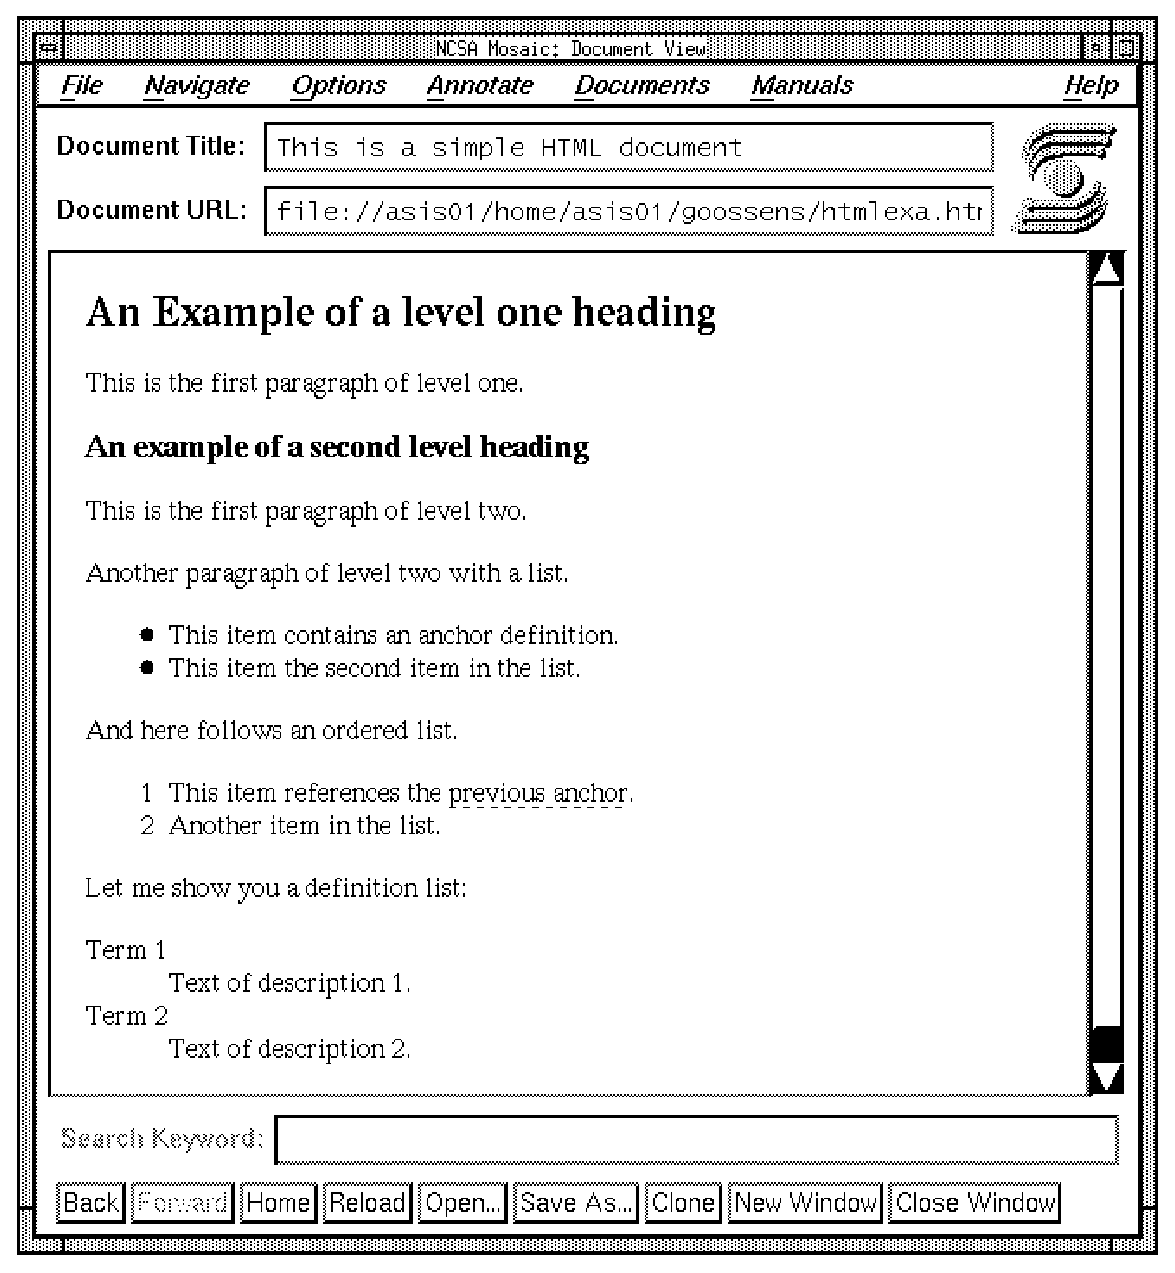
\epsfig{file=htmlexa.eps,width=\textwidth}
\caption{The output of the example \protect\Html{} source 
         shown by the \protect\Xmosaic{} program}
\label{fig:htmlexaoutxmosaic}
\end{minipage}
\end{minipage}
\end{sideways}
\end{figure}

Below we givew a tabular overview of some of the
more important commands, and their \LaTeX{} functional equivalent.

\begin{tabularx}{\textwidth}{@{}lXX@{}}
\textbf{Description}     & \textbf{\Html}       & \textbf{\LaTeX}                     \\
\textbf{Headings}        & \Lit{<H1>...</H1>}   & \Lcs{chapter}\Lit{\lcb...\rcb}      \\
                         & \Lit{<H2>...</H2>}   & \Lcs{section}\Lit{\lcb...\rcb}      \\
                         & \Lit{<H3>...</H3>}   & \Lcs{subsection}\Lit{\lcb...\rcb}   \\
                         & \Lit{<H4>...</H4>}   & \Lcs{subsubsection}\Lit{\lcb...\rcb}\\
                         & \Lit{<H5>...</H5>}   & \Lcs{paragraph}\Lit{\lcb...\rcb}    \\
                         & \Lit{<H6>...</H6>}   & \Lcs{subparagraph}\Lit{\lcb...\rcb} \\
\textbf{Lists}           & \Lit{OL}             & \LBEG{enumerate}                    \\ 
                         & \Lit{<LI>}           & \Lcs{item}                          \\ 
                         & \Lit{</OL>}          & \LEND{enumerate}                    \\
                         & \Lit{UL}             & \LBEG{itemize}                      \\ 
                         & \Lit{<LI>}           & \Lcs{item}                          \\ 
                         & \Lit{</UL>}          & \LEND{itemize}                      \\
                         & \Lit{DL}             & \LBEG{description}                  \\ 
                         & \Lit{<DT>...<DD>}    & \Lcs{item}\Lit{\lsb...\rsb}         \\
                         & \Lit{</DL>}          & \LEND{description}                  \\
\textbf{Specific markup} & \Lit{<P>}            & \Lcs{par}                           \\
                         & \Lit{<PRE>...</PRE>} & \Lit{\LBEG{XMP}...\LEND{XMP}}       \\
                         & \Lit{<EM>...</EM>}   & \Lit{\Lcs{textem}\lcb...\rcb}       \\
                         & \Lit{<SAMP>...</SAMP>}&\Lit{\Lcs{Lit}\lcb...\rcb}          \\
                         & \Lit{<KBD>...</KBD>} & \Lit{\Lcs{Ucom}\lcb...\rcb}         \\
\end{tabularx}

\subsection{Using hypertext link: defining and using anchors}

An anchor is a piece of text which marks the beginning and/or the
\index{anchor}\index{hypertext!link}
end of a hypertext link.   
   
The most two most important attributes of an anchor are:

\begin{XMP}
\fbox{<\textbf{A} HREF=\textem{link-name} NAME=\textem{link-def}>anchor text<\textbf{/A}>}
\end{XMP}

The text between the opening tag \Lit{<A>}
and the closing tag \Lit{</A>} is either the
start or destination (or both) of a link. 

The definition of these fields is:

\begin{DLtt}{1234}
\item[HREF] If the \Lit{HREF} attribute is present,
            the anchor is sensitive text, i.e., the start of a link. 
            If you select this text, you should be presented 
            with another document whose network address (\URL, or ``Universal 
            Resource Locator'') is defined by the value
            of the \Lit{HREF} attribute . 
            If you specify a form like \Lit{HREF="#identifier"}
            the you are referring to another anchor in the same document.
            Otherwise the anchor points to another document, and
            the attribute is a relative name , relative to
            the documents address. 
            An address like \Lit{HREF="docname#anchor"} specified an anchore
            inside the document ``\Lit{docname}''
\item[NAME] If present, the  attribute \Lit{NAME}
            allows the anchor to be the destination of a link.
            The value of the attribute is an unique arbitrary 
            string identifying the anchor.
            Another document can then reference this anchor (using the 
            \Lit{HREF} attribute,  by putting the identifier after the
            document address, separated by a hash sign . 
\end{DLtt}                         
\begin{XMPt}{Examples of anchors}

See <A HREF="http://info.cern.ch/">CERN</A>'s information for more details.

A <A NAME=WSdef>workstation</A> is a personal computer with a bitmap graphics 
screen, enough memory, computer power and disk space ...

Programmer productivity is increased when using a <a href="#WSdef">workstation</a>.
\end{XMPt}

\subsection*{Embedded images}

With \Html{} and viewers, which support the functionality, like
\Xmosaic{}, you can embed graphics images in your hypertext
documents.

You should use the \Lit{IMG} tag to include a small graphic image or an icon.
   
\begin{XMP}
\fbox{<\textbf{IMG} SRC=\Larg{graphURL} ALIGN=\Larg{aligment}>}
\end{XMP}
   
\begin{DLtt}{1234}
\item[SRC]   This is the \URL{} of the document to be embedded. 
             It has a syntax similar to that of the \Lit{HREF} attribute of
             the \Lit{<A>} tag. 
             The attribute is mandatory
\item[ALIGN] The optional attribute specifies the vertical alignment
             of the graphics with respect to the baseline of the 
             surrounding text.
             Possible values are \Lit{BOTTOM}, \Lit{MIDDLE} and \Lit{TOP}.
\end{DLtt}
                         
You can use \Lit{<IMG>} tags inside anchors.
   
Usually you will specify \gif{} images for embedded graphics.
Figure~\vref{fig:imgexample} shows the input and the resulting
output of a small \Html{} file containing a gif image vertically 
positioned in various ways.
In section~\ref{sec:epstogif} I shall explain how to generate
\gif{} image from \PS{} files.

\begin{figure}[p]
  \begin{sideways}
    \begin{minipage}[b]{0.999\textheight}%
\begin{minipage}[b]{.35\textwidth}
\small
\begin{verbatim}
<TITLE>Looking at images</TITLE>
<P>Text around CERN Logo 
   <IMG SRC="cernlogo.gif">
   Text around CERN Logo 
<P>xxxxx <IMG ALIGN=BOTTOM 
         SRC="cernlogo.gif">
   xxxxx <IMG ALIGN=TOP    
         SRC="cernlogo.gif">
   xxxxx
\end{verbatim}
\subfigure[Input \Html{} document]{\makebox[\textwidth]{}}% Dummy box for caption
\end{minipage} \hfill
\begin{minipage}[b]{.64\textwidth}
\subfigure[Viewing the document with \Xmosaic{}]{%
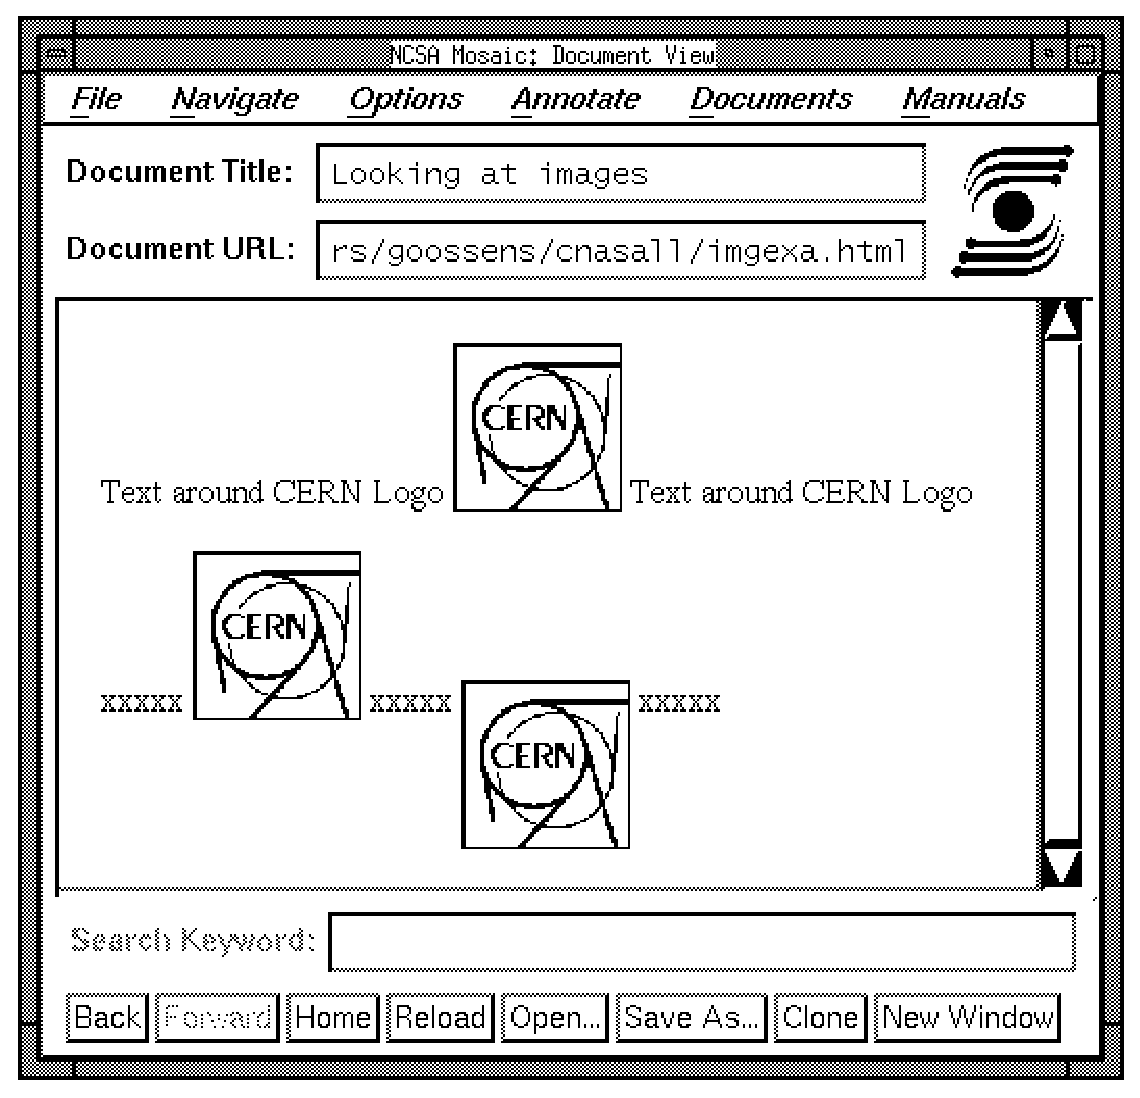
\epsfig{file=imgexa.eps,width=\textwidth}}
\end{minipage}
  \caption{Including \protect\gif{} images in \protect\Html{} documents}
  \label{fig:imgexample}
\end{minipage}
\end{sideways}
\end{figure}

\section{Using \protect\PTD}

The program \PTD{} converts a \Lit{.dvi} file into a plain text file.
It uses a slightly different approach from the popular \Lit{dvi2tty} program.
Instead of trying to position text without overlapping, \PTD{}
simply puts all characters into a two-dimensional grid (chars vs lines).
 
A special run of \LaTeX{} (i.e. using a dedicated style) is needed to
arrange the formatted text in a proper way.
This style (\Lit{cerndoc.sty}) not only maps all fonts onto the typewriter font,
but it also calculates the grid steps and adjusts all dimensions in
accordance with these steps.
A few macros (e.g. \Lcs{underline}, \Lcs{verb} are redefined too.
 
The \PTD{} program is primarily designed to generate on-line documentation
from
\LaTeX{} sources.
It has also been successfully used for the conversion of \LaTeX{} mark-up
to other tagging schemes, like SGML or HTML (for WWW).
 
The calling sequence of the program is:
\begin{verbatim}
      ptd [-dfpv]  file.dvi outfile
\end{verbatim}
 
The parameters have the following meaning:
\begin{DLtt}{12}
\item[-d]   debugging option;
\item[-f]   show font parameters;
\item[-p]   show preamble/postamble parameters;
\item[-v]   suppress warnings about replaced characters.
\end{DLtt}
 
 
As a design feature, the \PTD{} program will overwrite text. 
For example, when you reduce the \Lcs{baselineskip} parameter
inside a document, you will get a lot of warnings about 
characters being replaced.
The debug option is useful to locate where these replacements occur.
With this option active, the \PTD{} program prints a few lines in front
and following the point where the replacement occurs.
Note however, that the program does not care about 
the replacement of non-alphabetic characters, such as 
hyphens used for rendering rules.
 
\section[]{Supported \Lcs{special} commands}
 
\subsection*{\Lcs{special\{txtout: \Larg{argument}\}}}
 
This \Lcs{special} command recognizes the following fields:
 
\begin{DLtt}{1}
\item[H] horizontal step for the grid (in sp);
\item[V] vertical step for the grid (in sp);
\item[G] global offset (in characters);
\item[F] form feed flag.
\end{DLtt}
 
Usually this command is specified once before the first output.
The first two parameters are calculated by the style file
\Lit{cerndoc.sty} and supplied to \PTD{} via the following commands:
\begin{verbatim}
\newdimen\hquant   \newdimen\vquant
% the width of each letter in the font
\hquant=\the\fontdimen2\the\font
\ifcase \@ptsize
      \vquant=12pt
  \or \vquant=14pt
  \or \vquant=16pt
\fi
\newcount\along@h  \newcount\along@v
\along@h=\hquant   \along@v=\vquant
\special{textout: H:\the\along@h\space V:\the\along@v\space}
\end{verbatim}
 
The global offset is used as horizontal shift for the output
(by default there is no shift), e.g.
\begin{verbatim}
\special{textout: G:2} % shift everything two positions to the left
\end{verbatim}
 
If the form feed flag is present no form-feed character will be output
between pages (this character is output by default).
\begin{verbatim}
\special{textout: F:} % Don't separate pages by form feed
\end{verbatim}
 
\subsection*{\Lcs{special\{hidetext: \Larg{argument}\}}}
 
This kind of \Lcs{special} command
inserts the string \Larg{argument} into the output file
without affecting the formatted text.
It is very useful for embedding ``hidden'' commands, to be used e.g. by a
(hypertext) browser.
 
Assuming you need to specify an anchor which has  ``hot text'' (visible) and
a link (invisible ), then you can (e.g. using WWW's HTML syntax)
define a command \Lcs{anchor} with
two parameters: the hot text and the link.
 
\begin{verbatim}
\def\anchor#1#2{\special{hidetext:<A HREF=#2>}#1\special{hidetext:</a>}}
\end{verbatim}
 
You can use this command in WWW to include anchors, and
be sure that you do not affect the layout of the output page.
\begin{verbatim}
\anchor{My hot text}{http://info.cern.ch:80/mytext.html}
\end{verbatim}

\subsection{Creating gif files with gs and xv}
\label{sec:epstogif}


\addcontentsline{toc}{chapter}{Bibliography}
\bibliographystyle{myunsrt} % style for bibliography
\bibliography{/user/goossens/cnasall/cnasbibl}   % Master BibTeX file for CNAS docs
\addcontentsline{toc}{chapter}{Index}
\message{Index}
\input{\jobname.ind} % index

\end{document}



